\documentclass[12pt]{article}
\usepackage{amscd,amssymb,amsthm,amsxtra,exscale,latexsym,verbatim,paralist}
\usepackage{mathrsfs}
\usepackage[T1]{fontenc}
\usepackage{newtxmath,newtxtext}
\usepackage[margin=1in]{geometry}

%\usepackage{mathtools}
%\usepackage{multicol}
\usepackage{tikz}

\pagestyle{empty} 
\setlength{\parindent}{0pt} 
\setlength{\parskip}{\baselineskip}

\theoremstyle{plain}
\newtheorem{ex}{Exercise}

\renewcommand{\proofname}{Solution}

%\makeatletter
%\renewcommand*\env@matrix[1][*\c@MaxMatrixCols c]{%
%  \hskip -\arraycolsep
%  \let\@ifnextchar\new@ifnextchar
%  \array{#1}}
%\makeatother

\begin{document}

MTH 385 \qquad Homework due 2022-03-07

\begin{ex} [3.5.1]
  Explain the solution $x=21/4$, $y=71/8$ to $x^3-3x^2+3x+1=y^2$ given by Diophantus (Heath~(1910), p. 242) by constructing the tangent through the obvious rational point on this curve (Figure~3.4).
\end{ex}

\begin{center}
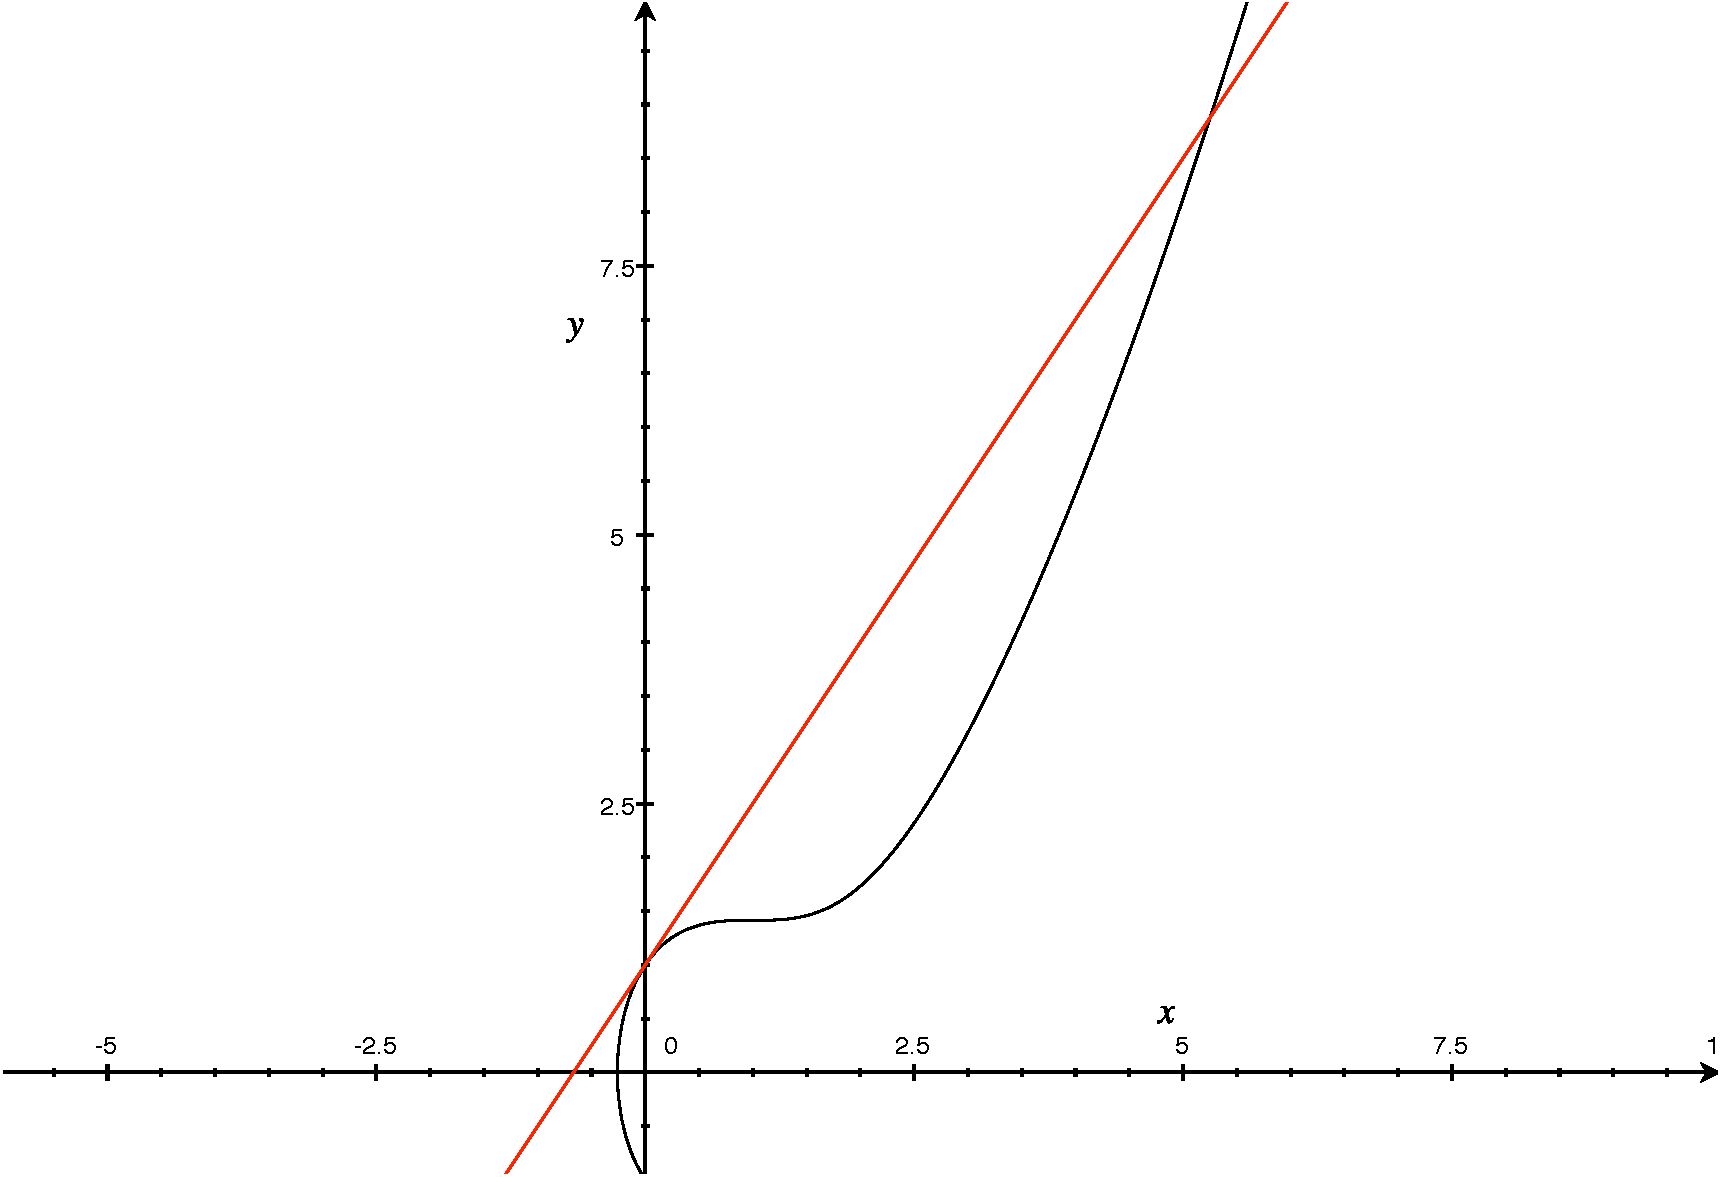
\includegraphics[scale=0.5]{cubic}

Figure~3.4: Cubic curve $y^2=x^3-3x^2+3x+1$ and tangent
\end{center}

\begin{ex} [3.5.2]
  Rederive the following rational point construction of Vi\`{e}te~(1593), p. 145. Given the rational point $(a,b)$ on $x^3-y^3=a^3-b^3$ , show that the tangent at $(a,b)$ is
  \[
    y=\frac{a^2}{b^2}(x-a)+b
  \]
  and that the other intersection of the tangent with the curve is the rational point
  \[
    x=a\frac{a^3-2b^3}{a^3+b^3},\qquad y=b\frac{b^3-2a^3}{a^3+b^3}.
  \]
\end{ex}

The \emph{Jade Mirror of Four Unknowns} does not go beyond four equations in four unknowns (hence the name). The idea is quite general, but it becomes hard to implement on the counting board when there are more than four unknowns. An amusing problem in three unknowns from the \emph{Jade Mirror}, which does not require the full strength of the elimination method, is given in the exercises below.

\begin{ex} [5.2.4]
  Problem~2 in the Jade Mirror (see Hoe~(1977), p. 135) is to find the side $a$ of a right-angled triangle $(a,b,c)$ such that
  \begin{align*}
    a^2-(b+c-a) &= ab, \\
    b^2+(a+c-b) &= bc.
  \end{align*}
  The \emph{Jade Mirror} suggests choosing the unknowns $x=a$ and $y=b+c$. Using $a^2=c^2-b^2$, show that this implies
  \begin{align*}
    b &= (y-x^2/y)/2, \\
    c &= (y+x^2/y)/2.
  \end{align*}
\end{ex}

\begin{ex} [5.2.5]
  Deduce that the first two equations in Exercise~5.2.4 are equivalent, respectively, to
  \begin{align*}
    (-2-x)y^2+(2x+2x^2)y+x^3  &= 0 \\
    (2-x)y^2+2xy+x^3          &= 0.
  \end{align*}
\end{ex}

\begin{ex} [5.2.6]
  By subtracting one equation in Exercise~5.2.5 from the other, deduce that $y=x^2/2$. Substitute this back to obtain a quadratic equation for $x$, with solution $x=a=4$. What are the values of $b$ and $c$?
\end{ex}

\end{document}

